\documentclass{beamer}

\usetheme{AAUsimple}

\usepackage{amsmath,amssymb,graphicx}
\usepackage{tikz}
\usetikzlibrary{arrows,decorations,decorations.markings}
\usepackage{listings}
\usepackage{upquote}
\newcounter{ipythoncounter}
\setcounter{ipythoncounter}{1}
\renewcommand{\ttdefault}{pcr}
\lstset{
  aboveskip=\bigskipamount,
  belowskip=\bigskipamount,
  basicstyle=\footnotesize\ttfamily,
  language=Python,
  numbers=left,
  stepnumber=9999,
  numberfirstline=true,
  xleftmargin=2cm,
}

\lstnewenvironment{ipythoninput} {
  \setcounter{lstnumber}{\value{ipythoncounter}} \renewcommand{\thelstnumber}
             {\bf\ttfamily In [\the\value{ipythoncounter}]:} \lstset{
               frame=single, frameround=tttt, name=ipythoninput, } } {
  \addtocounter{ipythoncounter}{1} }

\lstnewenvironment{ipythonoutput} { \addtocounter{ipythoncounter}{-1}
  \setcounter{lstnumber}{\value{ipythoncounter}} \renewcommand{\thelstnumber}
             {\bf\ttfamily Out[\the\value{ipythoncounter}]:} \lstset{
               name=ipythoninput } } { \addtocounter{ipythoncounter}{1} }

%% \newtheorem{theorem}{Theorem}
%% \newtheorem{definition}[theorem]{Definition}
%% \theoremstyle{definition}
%% \newtheorem{example}[theorem]{Example}

\DeclareMathOperator{\ZZ}{\mathbb{Z}}
\DeclareMathOperator{\RR}{\mathbb{R}}
\DeclareMathOperator{\CC}{\mathbb{C}}
\DeclareMathOperator{\hg}{\mathfrak{h}_g}
%% \DeclareMathOperator{\dx}{dx}
%% \DeclareMathOperator{\dt}{dt}
\newcommand{\dx}{\,\mathrm{d}x}
\newcommand{\dt}{\,\mathrm{d}t}
\newcommand{\dQ}{\,\mathrm{d}Q}
\DeclareMathOperator{\DivC}{\mathcal{C}}
\DeclareMathOperator{\DivD}{\mathcal{D}}
\DeclareMathOperator{\RCV}{\boldsymbol{K}}
\DeclareMathOperator{\Abel}{\boldsymbol{A}}
\DeclareMathOperator{\HalfLattice}{\Lambda_{1/2}}

\newcommand{\thchar}[2] {\begin{bmatrix}#1\\#2\end{bmatrix}}
\newcommand{\thcharsm}[2] {\left[ \begin{smallmatrix} #1
      \\ #2 \end{smallmatrix} \right]}



%%%%%%%%%%%%%%%%%%%%%%%%%%%%%%%%%%%%%%%%%%%%%%%%%%%%%%%%%%%%%%%%%%%%%%%%%%%%%%%
\title{Computing the Riemann Constant Vector}

\author{
  Chris Swierczewski\\
  {\tt cswiercz@uw.edu}
}

\date{21 April 2015}

\institute{
  Department of Applied Mathematics\\
  University of Washington\\
  Seattle, Washington
}

\pgfdeclareimage[height=1.5cm]{titlepagelogo}{AAUgraphics/aau_logo_new_circle}
\titlegraphic{
  \pgfuseimage{titlepagelogo}
}
%%%%%%%%%%%%%%%%%%%%%%%%%%%%%%%%%%%%%%%%%%%%%%%%%%%%%%%%%%%%%%%%%%%%%%%%%%%%%%%



%%%%%%%%%%%%%%%%%%%%%%%%%%%%%%%%%%%%%%%%%%%%%%%%%%%%%%%%%%%%%%%%%%%%%%%%%%%%%%%
\begin{document}
%%%%%%%%%%%%%%%%%%%%%%%%%%%%%%%%%%%%%%%%%%%%%%%%%%%%%%%%%%%%%%%%%%%%%%%%%%%%%%%

\begin{frame}[plain,noframenumbering]
  \titlepage
\end{frame}

\begin{frame}{Kadomtsev--Petviashvili Equation}{}
  $u(x,y,t) = $ surface height of a 2D periodic shallow water wave.
  \[
  \tfrac{3}{4} u_{yy} = \frac{\partial}{\partial x} \left(
  u_t - \tfrac{1}{4} \left(6uu_x + u_{xxx}\right) \right)
  \]

  \begin{columns}[T]
    \begin{column}{0.5\textwidth}
      \begin{figure}
        \centering
        \includegraphics[width=\textwidth]{images/livekp.jpg}
        \caption{\^{I}le de R\'{e}, France}
      \end{figure}
    \end{column}
    \begin{column}{0.5\textwidth}
      \begin{figure}
        \centering
        \includegraphics[width=\textwidth]{images/sd-harbor-model.jpg}
        \caption{Model of San Diego Bay}
      \end{figure}
    \end{column}
  \end{columns}

\end{frame}

\begin{frame}{Kadomtsev--Petviashvili Equation}{}
  ``Finite-genus solutions:''

  \vspace{12pt}

  \[
  u
  =
  c + 2 \partial_x^2 \log \theta\Big( \boldsymbol{U}x +
  \boldsymbol{V}y + \boldsymbol{W}t + \Abel\big(P^\infty,\DivD\big) -
  \RCV(P^\infty), \Omega \Big)
  \]

  \vspace{12pt}

  \pause

  \begin{itemize}[<+->]
  \item Riemann theta function $\theta : \CC^g \times \hg \to \CC$
    \[
    \theta(z,\Omega) = \sum_{n \in \ZZ^g} e^{2 \pi i
      \left(\tfrac{1}{2} n \cdot \Omega n + n \cdot z \right)}
    \]
  \item Quantities come from compact, connected, Riemann surfaces built from
    algebraic curves.
  \end{itemize}
\end{frame}


\begin{frame}{Whirlwind Background - Curves}{}
  Given $f \in \mathbb{C}[x,y]$ construct an {\it algebraic curve},
  \[
  C = \{ (\alpha, \beta) \in {\CC^*}^2 \; | \; f(\alpha, \beta) = 0 \}.
  \]

  \pause

  $C$ as a {\it $y$-covering} of $\CC_x^*$:
  \begin{itemize}[<+->]
    \item For each $x \in \CC$, what are all possible $y$-roots to $f(x,y)=0$?
      \[
          x \mapsto y(x) = (y_1(x), \ldots, y_d(x))
      \]
    \item $y_i$'s are continuous functions of $x$
  \end{itemize}

  \pause

  \begin{block}{Question}
    As $x \in \CC_x^*$ varies on what surface is $y$ single-valued?
  \end{block}
\end{frame}


\begin{frame}{Whirlwind Background - Riemann Surfaces}{}
  (Compact) Riemann Surfaces $X$:

  \begin{itemize}[<+->]
    \item connected, 1-dimensional complex manifold,
    \item homeomorphic to a doughnut with $g$ holes,
      \begin{itemize}
        \item $g$ = {\it genus}
      \end{itemize}
    \item surface on which $y(x)$ is single-valued,
      \begin{itemize}
        \item (branch cuts, etc.)
        \item (caveats: singular points and points at infinity)
        \item (optional board demo for undergraduates)
      \end{itemize}
  \end{itemize}
\end{frame}


\begin{frame}{Whirlwind Background - Homology}{}
  \begin{figure}
  \centering
  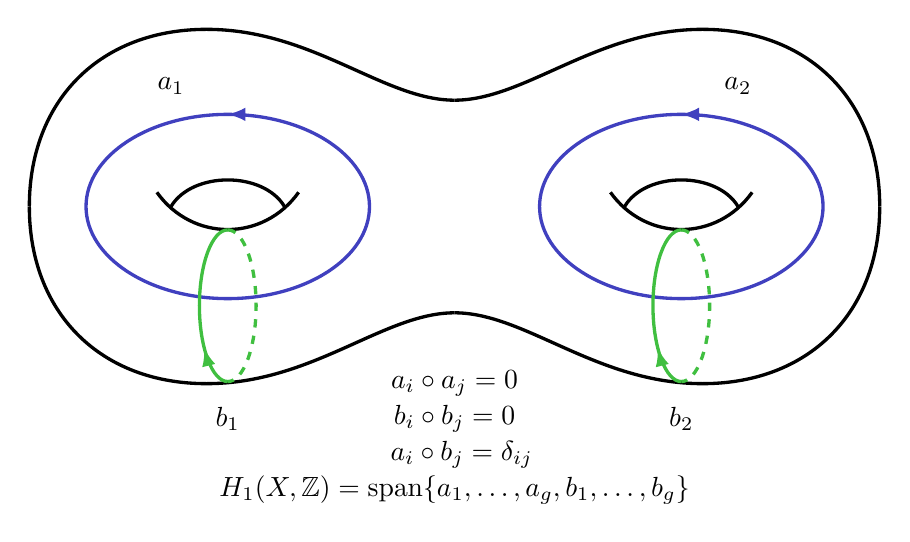
\begin{tikzpicture}[scale=0.9]
    \colorlet{darkgreen}{green!50!gray}
    \colorlet{lightgray}{white!80!black}
    \colorlet{darkblue}{blue!50!gray}

    %% % Bezier Control Points
    %% \filldraw [gray] (-6,0) circle (2pt)
    %%                  (-6,1.5) circle (2pt)
    %%                  (-5,2.5) circle (2pt)
    %%                  (-3.5,2.5) circle (2pt)
    %%                  (-2,2.5) circle (2pt)
    %%                  (-1,1.5) circle (2pt)
    %%                  (0,1.5) circle (2pt);


    % the reference volume
    %\draw[lightgray, thick]         (0,-1.5) arc (270:90:0.4cm and 1.5cm);
    %\draw[lightgray, thick, dashed] (0,1.5)  arc (90:-90:0.4cm and 1.5cm);

    \begin{scope}[very thick]
    % Quadrant II of Torus
    % (other draw statements are flips / rotations)
    \draw (-6,0) ..
          controls (-6,1.5) and (-5,2.5) ..
          (-3.5,2.5) ..
          controls (-2,2.5) and (-1,1.5) ..
          (0,1.5);
    \draw[xscale=-1] (-6,0) ..
          controls (-6,1.5) and (-5,2.5) ..
          (-3.5,2.5) ..
          controls (-2,2.5) and (-1,1.5) ..
          (0,1.5);
    \draw[rotate=180] (-6,0) ..
          controls (-6,1.5) and (-5,2.5) ..
          (-3.5,2.5) ..
          controls (-2,2.5) and (-1,1.5) ..
          (0,1.5);
    \draw[yscale=-1] (-6,0) ..
          controls (-6,1.5) and (-5,2.5) ..
          (-3.5,2.5) ..
          controls (-2,2.5) and (-1,1.5) ..
          (0,1.5);

    % The Holes
    % (one hole at center shifted to outsides)
    \draw[xshift=-3.2cm] (-0.8,0) ..
          controls (-0.5,0.5) and (0.5,0.5) ..
          (0.8,0);
    \draw[yscale=-1,xshift=-3.2cm] (-1,-0.2) ..
          controls (-0.5,0.5) and (0.5,0.5) ..
          (1,-0.2);

    \draw[xshift=3.2cm] (-0.8,0) ..
          controls (-0.5,0.5) and (0.5,0.5) ..
          (0.8,0);
    \draw[yscale=-1,xshift=3.2cm] (-1,-0.2) ..
          controls (-0.5,0.5) and (0.5,0.5) ..
          (1,-0.2);

    \pause

    % a-cycles
    \draw[xshift=-3.2cm, darkblue, decoration={markings,
              mark=at position 0.25 with {\arrow[very thick]{latex}}},
          postaction={decorate}]
         (0,0) ellipse (2cm and 1.3cm);
    \draw[xshift=3.2cm, darkblue, decoration={markings,
              mark=at position 0.25 with {\arrow[very thick]{latex}}},
          postaction={decorate}]
         (0,0) ellipse (2cm and 1.3cm);

    % b-cycles
    \draw[xshift=-3.2cm, yshift=-2.47cm,
          darkgreen, decoration={markings,
              mark=at position 0.25 with {\arrow[very thick]{latex}}},
          postaction={decorate}]
         (0,0) arc (270:90:0.4cm and 1.07cm);
    \draw[xshift=-3.2cm, yshift=-0.33cm, dashed, darkgreen]
         (0,0) arc (90:-90:0.4cm and 1.07cm);
    \draw[xshift=3.2cm, yshift=-2.47cm,
          darkgreen, decoration={markings,
              mark=at position 0.25 with {\arrow[very thick]{latex}}},
          postaction={decorate}]
         (0,0) arc (270:90:0.4cm and 1.07cm);
    \draw[xshift=3.2cm, yshift=-0.33cm, dashed, darkgreen]
         (0,0) arc (90:-90:0.4cm and 1.07cm);

    % cycle labels
    \draw (-4,1.7)  node {$a_1$};
    \draw (4,1.7)   node {$a_2$};
    \draw (-3.2,-3) node {$b_1$};
    \draw (3.2,-3)  node {$b_2$};


    % cycle intersection properties
    \draw (0,-2.5)   node {$a_i \circ a_j = 0$};
    \draw (0,-3) node {$b_i \circ b_j = 0$};
    \draw (0.1,-3.5) node {$a_i \circ b_j = \delta_{ij}$};
    \draw (0,-4) node
    {$H_1(X,\mathbb{Z}) = \text{span}\{a_1,\ldots,a_g,b_1,\ldots,b_g\}$};

    \end{scope}
  \end{tikzpicture}
  \end{figure}
\end{frame}


\begin{frame}{}{}
  \vspace{32pt}
  \begin{center}
    {\Huge \it Demo}

    \vspace{24pt}

    Homology Basis
  \end{center}
\end{frame}


\begin{frame}{Whirlwind Background - One-Forms}{}
  \begin{block}{Question}
    What do we usually do with paths?
  \end{block}

  \pause

  \begin{block}{Answer}
    Integrate ``things'' on them.
  \end{block}

  \pause

  Meromorphic one-forms on $X$
  \[
      \nu \in \Omega_X^1,
  \]

  \pause

  %% For each neighborhood $U \subset X$ with ``local coordinate'' $t$, $\nu$ is
  %% locally written as
  %% \[
  %%     \nu \Big|_{U} =
  %%     h\big(t)dt, \quad h \text{ meromorphic}.
  %% \]
  On $C$ they look like
  \[
  \nu = \nu(x,y) \dx
  \]
\end{frame}

\begin{frame}{Whirlwind Background - One-Forms}{}
  Consider only $\omega \in \Omega_X^1$ {\it holomorphic} on $X$

  \pause

  %% \[
  %% \omega \Big|_{U} =
  %% h\big(t)dt, \quad h \text{ holomorphic}.
  %% \]
  \[
  \omega = \omega(x,y) \dx
  \]

  \pause

  {\it ``Abelian differentials of the first kind''}
  \[
  \Gamma(X,\Omega_X^1)
  \]

  \begin{block}{Theorem}
    \[
    \Gamma(X,\Omega_X^1)
    =
    \text{span}_{\CC[x,y]} \{ \omega_1, \ldots, \omega_g \}
    \]
  \end{block}
\end{frame}


\begin{frame}{Whirlwind Background - One-Forms}{}
  \begin{block}{Theorem}
    \[
    \Gamma(X,\Omega_X^1)
    =
    \text{span}_{\CC[x,y]} \{ \omega_1, \ldots, \omega_g \}
    \]
  \end{block}
  \begin{itemize}[<+->]
  \item ``normalized'' basis $\{ \omega_i \}$ is such that
    \[
    \oint_{a_j} \omega_i = \delta_{ij}
    \]
  \item algorithm returns a non-normalized basis
    \[
    \{ \tilde{\omega}_1, \ldots, \tilde{\omega}_g \}
    \]
  \end{itemize}
\end{frame}


\begin{frame}{}{}
  \vspace{32pt}
  \begin{center}
    {\Huge \it Demo}

    \vspace{24pt}

    Abelian differentials of the first kind
  \end{center}
\end{frame}


\begin{frame}{Whirlwind Background - Period Matrix}{}
  Culmination of the theory: construct matrices
  \[
  \oint_{a_j} \omega_i = \delta_{ij}, \qquad
  \oint_{b_j} \omega_i = \Omega_{ij}
  \]

  \pause

  The matrix $\Omega \in \CC^{g \times g}$ is a {\it ``Riemann matrix''}
  \begin{itemize}[<+->]
  \item symmetric
  \item $\text{Im}(\Omega) > 0$
  \end{itemize}

  \pause

  Non-normalized differentials
  \[
  \oint_{a_j} \tilde{\omega}_i = A_{ij}, \qquad
  \oint_{b_j} \tilde{\omega}_i = B_{ij}
  \]

  \pause

  \begin{center}
  Fact: $\Omega = A^{-1}B$
  \end{center}
\end{frame}


\begin{frame}{Whirlwind Background - Period Matrix}{}
  Period matrix
  \[
  \tau = [I \; \; \Omega] \in \CC^{g \times 2g}
  \]

  \pause

  Jacobian of the Riemann surface
  \[
  J(X) = \CC^g / \Lambda
  \]
  where
  \[
  \Lambda = \ZZ^g \times \, \Omega \ZZ^g
  \]
\end{frame}

\begin{frame}
  \vspace{32pt}
  \begin{center}
    {\Huge \it Demo}

    \vspace{24pt}

    Period matrix
  \end{center}
\end{frame}


\begin{frame}{Whirlwind Background - Places and Divisors}{}
  A {\it place} $P \in X$ can be represented locally by a ``Puiseux series''
  \[
  P =
  \begin{cases}
    x_P(t) = \alpha + \lambda t^e, \\
    y_P(t) = \sum_{k=0}^\infty \beta_k t^{n_k},
  \end{cases}
  \]

  \pause

  \begin{itemize}[<+->]
  \item $e = $ {\it ramification index}
  \item places {\it lie above} the curve $C$
    \[
    P \big|_{t=0} = (\alpha, \beta) \in C
    \]
  \item there can be distinct places with same projection on $C$.
  \end{itemize}
\end{frame}


\begin{frame}{Whirlwind Background - Places and Divisors}{}
  A {\it divisor} $\DivD$ on $X$ is a finite formal linear comb. of places
  \[
  \DivD = \sum n_i P_i
  \]

  \pause

  \begin{itemize}[<+->]
  \item $\deg \DivD = \sum_i n_i$
  \item $\text{Div}(X)$ is an Abelian group
  \item {\it effective} if $\forall i, n_i \geq 0$
  \end{itemize}

  \pause

  \begin{block}{Valuation Divisors}
    Given $\nu \in \Omega_X^1$,
    \[
    (\nu)_\text{val} = \sum_{i=1}^m p_iP_i - \sum_{j=1}^n q_jQ_j
    \]
    is called the {\it valuation divisor} of $\nu$
  \end{block}

  \pause

  $\DivC \in \text{Div}(X)$ is {\it canonical} if $\DivC$ is a valuation
  divisor
\end{frame}


\begin{frame}{}{}
  \vspace{32pt}
  \begin{center}
    {\Huge \it Demo}

    \vspace{24pt}

    Places and divisors
  \end{center}
\end{frame}




%------------------------------------------------------------------------------
\section*{Abel Map}
%------------------------------------------------------------------------------

\begin{frame}{The Abel Map}{}

  Let $P \in X$ be a fixed place. The Abel Map
  \[
  \Abel : X \to J(X)
  \]

  \pause

  is defined by
  \[
  \Abel(P,Q) = \big( A_1(P,Q), \ldots, A_g(P,Q) \big),
  \]
  where
  \[
  A_j(P,Q) = \int_P^Q \omega_j.
  \]

  \pause

  \begin{block}{Abel Map on Divisors}
    If $\DivD = \sum_i n_i P_i$ then
    \[
    \Abel(P,\DivD) = \sum_i n_i \bold \Abel(P,P_i)
    \]
  \end{block}
\end{frame}


\begin{frame}
  \vspace{32pt}
  \begin{center}
    {\Huge \it Demo}

    \vspace{24pt}

    The Abel Map
  \end{center}
\end{frame}


\begin{frame}{Riemann Constant Vector}
  The Riemann constant vector
  \[
  \RCV : X \to J(X)
  \]

  \pause

  is defined as
  \[
  \RCV(P) = \big( K_1(P), \ldots, K_g(P) \big),
  \]
  where
  \[
  K_j(P) = \frac{1 + \Omega_{jj}}{2} - \sum_{k \neq j}^g
           \oint_{a_k} \omega_k(Q) A_j(P,Q) \dQ.
  \]
\end{frame}


\begin{frame}{Riemann Constant Vector}
  \[
  K_j(P) = \frac{1 + \Omega_{jj}}{2} - \sum_{k \neq j}^g
           \oint_{a_k} \omega_k(Q) A_j(P,Q) \dQ
  \]

  \begin{itemize}
  \item Double integral: difficult to compute.
  \end{itemize}

  \pause

  \begin{block}{Theorem}
    Let $P_0,P \in X$. Then
    \[
    \RCV(P) = \RCV(P_0) + (g-1)\Abel(P_0,P).
    \]
  \end{block}

  \pause

  \begin{itemize}
  \item Idea: most work from computing $\RCV(P_0)$ \underline{once}.
  \end{itemize}
\end{frame}

\begin{frame}{Computing the RCV}{}

  \vspace{12pt}

  Algorithm to compute $\RCV(P_0)$ inspired by two theorems:

  \pause

  \vspace{24pt}

  \begin{block}{Theorem}
    \alt<2>{
      Let $\DivC$ be a divisor of degree $2g-2$. Then $\DivC$ is a
      canonical divisor if and only if
      \[
      2 \RCV(P_0) \equiv - \Abel(P_0,\DivC).
      \]
      \vspace{4in}
    }{
      A vector $\boldsymbol{W} \in J(X)$ satisfies
      \[
      \theta(\boldsymbol{W}, \Omega) = 0,
      \]
      if and only if $\exists \DivD = P_1 + \cdots + P_{g-1}$ such that
      \[
      \boldsymbol{W} = \Abel(P_0,\DivD) + \RCV(P_0).
      \]
      \vspace{4in}
    }
  \end{block}
  \visible<3->{}
\end{frame}


\begin{frame}{Computing the RCV}{}
  Combining the theorems:
  \begin{enumerate}[<+->]
  \item compute a canonical divisor $\DivC$,
  \item solve the equation
    \[
    2 \RCV(P_0) \equiv - \Abel(P_0,\DivC),
    \]
  \end{enumerate}
\end{frame}


\begin{frame}{1. Computing a Canonical Divisor}{}
  Meromorphic differential:
  \[
  \nu = \frac{p(x,y) \dx}{q(x,y)}
  \]

  \pause

  \vspace{12pt}

  Valuation divisor:
  \[
  (\nu)_\text{val} = \sum_i p_i P_i - \sum_j q_j Q_j
  \]
\end{frame}


\begin{frame}{1. Computing a Canonical Divisor}{}
  Given $P \in X$, \\
  \[
  P = \big( x_P(t), y_P(t) \big),
  \]

  \vspace{12pt}
  a \underline{necessary} condition for $P \in (\nu)_\text{val}$ is \\

  \begin{align*}
    p\big(x_P(t), y_P(t)\big) \Big|_{t=0} \! &= 0, \\
    \qquad
    q\big(x_P(t), y_P(t)\big) \Big|_{t=0} \! &= 0, \quad or \\
    \frac{\dx_P}{\dt}\big(0\big) = x_P'(t)dt \Big|_{t=0} &= 0.
  \end{align*}
\end{frame}


\begin{frame}
  \vspace{32pt}
  \begin{center}
    {\Huge \it Demo}

    \vspace{24pt}

    Localizing Differentials at Places
  \end{center}
\end{frame}


\begin{frame}{1. Computing a Canonical Divisor}{}
  {\bf Goal:} find $\mathcal{P}$ containg the places in $(\nu)_\text{val}$.

  \pause

  \vspace{12pt}

  Use ``resultant sets'':
  \begin{itemize}[<+->]
  \item $R(f,p)(x) = $ resultant of $f(x,y)$ and $p(x,y)$ w.r.t. $y$,
  \item roots of $R$ are $\alpha \in \CC_x$ such that
    \[
    f(\alpha,y) = 0 \quad \text{and} \quad p(\alpha,y) = 0
    \]
    have simultaneous solutions,
  \item {\bf The point:} $P=(x_P(t),y_P(t))$ is a zero of $p(x,y)$ only if
    $x_P(0)$ is a root of $R(f,p)$,
  \end{itemize}

\end{frame}


\begin{frame}{1. Computing a Canonical Divisor}{}
  Given
  \[
  \nu = \frac{p(x,y) \dx}{q(x,y)}
  \]
  Define
  \[
  \begin{aligned}
    \action<+->{
      \mathcal{X}_\nu^{(1)}
      &=
      \left\{ \alpha \in \CC \; | \; R(f,p)(\alpha)=0 \right\} \\
    }
    \action<+->{
      \mathcal{X}_\nu^{(2)}
      &=
      \left\{ \alpha \in \CC \; | \; R(f,q)(\alpha)=0 \right\} \\
    }
    \action<+->{
      \mathcal{X}_\nu^{(3)}
      &=
      \left\{ \alpha \in \CC \; | \; \alpha \text{ is a branch point of } f \right\} \\ \phantom{x} \\
    }
    \action<+->{
      \mathcal{X}_\nu
      &=
      \mathcal{X}_\nu^{(1)}
      \cup
      \mathcal{X}_\nu^{(2)}
      \cup
      \mathcal{X}_\nu^{(3)}
      \cup
      \{ \infty \} \\ \phantom{x} \\
    }
    \action<+->{
      \mathcal{P}
      &=
      \left\{ P \in X \; | \; x_P(0) \in \mathcal{X}_\nu \right\}
    }
  \end{aligned}
  \]
\end{frame}

\begin{frame}{1. Computing a Canonical Divisor}{}
  \begin{block}{Optimization}
  Use the Abelian differentials of the 1st kind:
  \[
  \tilde{\omega}_i = \frac{p_i(x,y) \dx}{\partial_y f(x,y)}
  \]
  \end{block}

  \begin{itemize}[<+->]
  \item already computed the $\tilde{\omega}_i$'s,
  \item already computed roots of $R(f,\partial_y f)(x)$, (branch points)
  \item $p_i$'s tend to be simple monomials,
  \item no poles $\to$ terminate when $\deg$ reaches $2g-2$,
  \end{itemize}
\end{frame}


\begin{frame}
  \vspace{32pt}
  \begin{center}
    {\Huge \it Demo}

    \vspace{24pt}

    Computing a Canonical Divisor
  \end{center}
\end{frame}


\begin{frame}{2. Finding the Half-Lattice Vector}{}
  Solve for $\RCV(P_0)$
  \[
  2\RCV(P_0) \equiv - \Abel(P_0,\DivC)
  \]

  \pause

  Embed into $\CC^g$
  \[
  2\RCV(P_0) + \Abel(P_0,\DivC) = \boldsymbol{\lambda}
  \]
  where
  \[
  \boldsymbol{\lambda} \equiv \boldsymbol{0} \bmod{\Lambda}
  \]
  \begin{block}{Embed in $\CC^g$}
    $\boldsymbol{\lambda}$ is one of the $2^{2g}$ lattice vectors in the
    fundamental region of $\Lambda$.
  \end{block}
\end{frame}


\begin{frame}{2. Finding the Half-Lattice Vector}{}
  Division by two is legal in $\CC^g$
  \[
  \RCV(P_0) = \boldsymbol{h} - \tfrac{1}{2}\Abel(P_0,\DivC)
  \]
  where $\boldsymbol{h} = \boldsymbol{\lambda}/2$ is one of $2^{2g}$ {\it
    half-lattice vectors}

  \pause

  \vspace{12pt}

  Project down to $J(X) = \CC^g / \Lambda$
  \[
  \RCV(P_0) \equiv \boldsymbol{h} - \tfrac{1}{2}\Abel(P_0,\DivC)
  \]

  \pause

  \begin{block}{Goal}
    Find an appropriate half-lattice vector $\boldsymbol{h}$.
  \end{block}
\end{frame}

\begin{frame}{2. Finding the Half-Lattice Vector}{}
  \begin{block}{Theorem}
    For any effective, degree $g-1$ divisor $\DivD = P_1 + \cdots + P_{g-1}$,
    \[
    \theta \big( \Abel(P_0,\DivD) + \RCV(P_0), \Omega \big) = 0.
    \]
  \end{block}

  \pause

  Consider the divisor $\DivD = (g-1)P_0$. Then
  \[
  \begin{aligned}
    \action<+->{
      \theta\big(\Abel(P_0,\DivD) + \RCV(P_0), \Omega \big)
      &=
      \theta\Big(\Abel\big(P_0,(g-1)P_0\big) + \RCV(P_0), \Omega \Big) \\
    }
    \action<+->{
      &=
      \theta\Big( (g-1) \Abel\big(P_0,P_0\big) + \RCV(P_0), \Omega \Big) \\
    }
    \action<+->{
      &=
      \theta\big(\boldsymbol{0} + \RCV(P_0), \Omega \big) \\
    }
    \action<+->{
      &=
      \theta\big(\RCV(P_0), \Omega \big) \\
    }
    \action<+->{
      &= 0
    }
  \end{aligned}
  \]
\end{frame}


\begin{frame}{2. Finding the Half-Lattice Vector}{}
  \begin{block}{The Point}
    It is necessary that
    \[
    \theta \big(
    \boldsymbol{h}_j - \tfrac{1}{2} \Abel(P_0,\DivC), \Omega
    \big) = 0
    \]
    for {\it at least one} of the $2^{2g}$ half lattice vectors
    $\boldsymbol{h}_j$.
  \end{block}

  \pause

  \begin{block}{Basic Strategy}
    Evaluate above espression with each $\boldsymbol{h}_j$ to find a zero.
  \end{block}

  \pause

  \begin{block}{Conjecture}
    This only works for {\it exactly one} $\boldsymbol{h}_j$.
  \end{block}

\end{frame}

\begin{frame}{2. Finding the Half-Lattice Vector}{}
  Numerical considerations:
  \begin{itemize}[<+->]
  \item $\theta$ computation accurate to order $\epsilon$ (at best machine
    precision)
  \item only use ``oscillatory part'' of $\theta$
  \item filter out any $\boldsymbol{h}_j$ such that
    \[
    \bigg|
    \theta \big(
    \boldsymbol{h}_j - \tfrac{1}{2} \Abel(P_0,\DivC), \Omega
    \big)
    \bigg| > \epsilon
    \]
  \item continue filtering by shifting by $\Abel(P_0,\DivD)$
    \[
    \bigg|
    \theta \big(
    \boldsymbol{h}_j - \tfrac{1}{2} \Abel(P_0,\DivC) + \Abel(P_0,\DivD), \Omega
    \big)
    \bigg| > \epsilon
    \]
    (for any degree $g-1$ effective divisor $\DivD$)
  \end{itemize}
\end{frame}


\begin{frame}
  \vspace{32pt}
  \begin{center}
    {\Huge \it Demo}

    \vspace{24pt}

    Finding a half-lattice vector. Verifying results.
  \end{center}
\end{frame}


\begin{frame}{Concluding Remarks and Next Steps}{}
  Solutions to KP:
  \begin{overprint}
  \onslide<1>
  \[
  u = c + 2 \partial_x^2 \log \theta\Big(
  \boldsymbol{U}x + \boldsymbol{V}y + \boldsymbol{W}t
  + \Abel\big(P^\infty, \DivD\big) -
  \RCV(P^\infty)
  , \Omega \Big),
  \]

  \onslide<2>
  \[
  u = c + 2 \partial_x^2 \log \theta\Big(
  \boldsymbol{U}x + \boldsymbol{V}y + \boldsymbol{W}t
  + \Abel\big(P^\infty, \DivD\big) -
  \underbrace{
    \RCV(P^\infty)}_\text{now have this}
  , \Omega \Big),
  \]

  \onslide<3>
  \[
  u = c + 2 \partial_x^2 \log \theta\Big(
  \underbrace{
    \boldsymbol{U}x + \boldsymbol{V}y + \boldsymbol{W}t}_\text{remaining work}
  + \Abel\big(P^\infty, \DivD\big) -
  \underbrace{
    \RCV(P^\infty)}_\text{now have this}
  , \Omega \Big),
  \]

  \end{overprint}
\end{frame}


\begin{frame}
  \vspace{32pt}
  \begin{center}
    {\Huge Thank You!}

    \vspace{24pt}

    {cswiercz@uw.edu}

    \vspace{12pt}

    {http://abelfunctions.cswiercz.info}
  \end{center}
\end{frame}




%%%%%%%%%%%%%%%%%%%%%%%%%%%%%%%%%%%%%%%%%%%%%%%%%%%%%%%%%%%%%%%%%%%%%%%%%%%%%%%
\end{document}
%%%%%%%%%%%%%%%%%%%%%%%%%%%%%%%%%%%%%%%%%%%%%%%%%%%%%%%%%%%%%%%%%%%%%%%%%%%%%%%
